\section*{Reproducibility Summary}


\subsubsection{Scope of Reproducibility}
In this work, we aim to reproduce the findings of the paper "Optimizing Deep Learning Inference on Embedded Systems Through Adaptive Model Selection"\supercite{marco2019optimizing}. The paper presents a set of methods for improving deep learning inference on power-constrained systems, aiming to utilise a simple premodel (KNN, SVM, DT) to determine the optimal (in this case least power-intensive) model for each input.

\subsubsection{Methodology}
We discovered a partial implementation in an archived GitHub repository, which only covered the computer vision aspect of the study. However, this was insufficient for full reproduction of the results, leading us to implement the majority of the code from scratch.

\subsubsection{Results}
Our results differ significantly from the original article, due to their inability to provide specific information about the methods and decisions made in the implementation phase. Although we were able to achieve similar correlation in the feature engineering and premodel parts, the differences in subsequent parts grew quickly. Despite achieving similar top-end performance in the premodel and image classification part, the accuracy of NLP models did not match our expectations. Thus we unable to fully reproduce the results of the original article.

\subsubsection{What was easy}
%The easiest task was writing the code itself - the source idea is relatively simple to implement.
Implementing the core idea in code was relatively straightforward, as the foundational concepts were clear and simple to execute.

\subsubsection{What was difficult}
It was very difficult to understand what values and procedures the original authors used to procure their results for model selection, feature engineering and model training. Specifically, the lack of explicitly stated methods used for feature engineering and only referencing an overview study of the subject. Furthermore, for premodel results, the only reported accuracy values were in comparison to oracle performance, which was stated nowhere in the original article. 

\subsubsection{Communication with original authors}
%We attempted to contact the original authors about their results over email, listed in their original article, however no response was received. -> We contacted the aouthors via email listed in the original paper, but they did not respond.

We contacted the authors via email listed in the original paper, but they did not respond.



\section{Introduction}
Deep learning produces models capable of performing a wide range of complex tasks. However, such models tend to consume a lot of computing power, which is often a limiting factor for using them on embedded systems. While less power-intense models exist, they tend to give less accurate results or even completely fail at harder problems.

Marco et. al. \cite{marco2019optimizing} propose an adaptive model selection method to leverage less power-intense models for simple tasks while employing more powerful models to achieve good results even on complex tasks.

Here we attempt to reproduce their work on the two DNN domains described in the paper: image classification and machine translation.

\section{Scope of Reproducibility}
Authors have the following claims:
\begin{itemize}
	\item \textbf{Claim 1: image classification top-1 accuracy improvement.}
	      
	      The authors claim that, using the premodel selection pipeline, we can surpass the accuracy of any one of pretrained networks. They state an improvement of 7.52\% compared to the most-accurate single deep learning model.
	      
	\item \textbf{Claim 2: image classification reduction in inference time.}
	    %Scope of reproduciblity, Claim2: Čudni narekovaji (če imamo te ukrivljene, moramo imeti '' in ´´, ne?). Pa zakaj imamo tu v narekovajih, pri Claim 3 pa podobnega stavka ne?
	      %The authors claim that using the premodels, we can reduce the inference time by more than half ("1.8x reduction in inference time") that of using only the most accurate model - ResNet152.
       The authors claim that using the premodels, we can achieve a 1.8x reduction in inference time, compared to using only the most accurate model - ResNet152.
	      
	\item \textbf{Claim 3: machine translation reduce inference time without affecting accuracy.}
	      
	      The authors claim a 1.34x reduction in inference time without a significant loss in accuracy.
	      
\end{itemize}


\section{Methodology}

Our replication effort focused on the adaptive model selection methodology, particularly for image classification and machine translation tasks. To compensate for the absence of official code from the original study, we referred to an \href{https://github.com/qwerybot/Adaptive_Deep_Learning}{archived GitHub repository}, which was related to a previous study\supercite{taylor2018adaptive} by the same authors. This earlier study concentrated specifically on the image classification aspect.

Our approach involved adapting the available resources and developing custom methodologies where necessary. For image classification, we devised our own feature extraction and premodel techniques, drawing insights from the descriptions in the referenced papers. In the area of machine translation, we tackled the challenges posed by dataset discrepancies and the lack of specific methodological details in the original paper.

The objective was to closely emulate the experimental setup of the original study, making informed adaptations to fill in the gaps where explicit details were not provided.

\subsection{Image classification}

Our efforts in the image classification section were focused on the premodel construction and comparison, as the pretrained image classification neural networks are freely available online, and as such require no reproducibility testing.
\paragraph{Architecture}
The chosen model selector architectures were 16-depth decision tree, a support vector classifier and a K-nearest-neighbours classifier. These were combined into a 3-layer hierarchy, where each further layer only classified those datapoints that the previous ones did not.
\paragraph{Comparison}
The premodel combinations were compared in inference time, as model construction is a pre-processing step and does not affect real-world performance. Furthermore, they were compared in top-1 accuracy versus a hypothetical ideal model selector - referred to as the Oracle.


\subsubsection{Premodel}
In the original paper, the premodel is constructed with three consecutive simple models, to estimate large neural network performance. Specifically, quick model selection among 4 pre-trained image-classification neural network models - specifically \textit{mobilenet v1, resnet50 v1, inception v2, and resnet 152 v2}. As per the original authors, we tested all configurations of the three premodel variations on different hierarchy levels, ensuring performance with 10-fold cross-validation.

For comparison, runtime and accuracy as they report it is shown in Figure \ref{fig:11a_orig}, while our results are shown in Figure \ref{fig:11a_ours}. Some of these differences could be attributed to the lack of clear information on what features the authors used, and how they were extracted or augmented.

%Figure 1: A to je prav iz originalnega članka? Dajte si malo pogledat, pod kakšno licenco je originalni članek. Če je copyrighted, je načeloma potrebno pridobiti soglasje. Worst case se morate sklicevati na ta figure v originalnem članku in ga ne imeti v članku.

%Original na arXiv u uporablja licenco CC4.0 (apparently se licence pogleda pod download gumbi na arXivu) - we are free to redistribute, share and edit, as long as we tell that we did

\begin{figure}
	\centering
	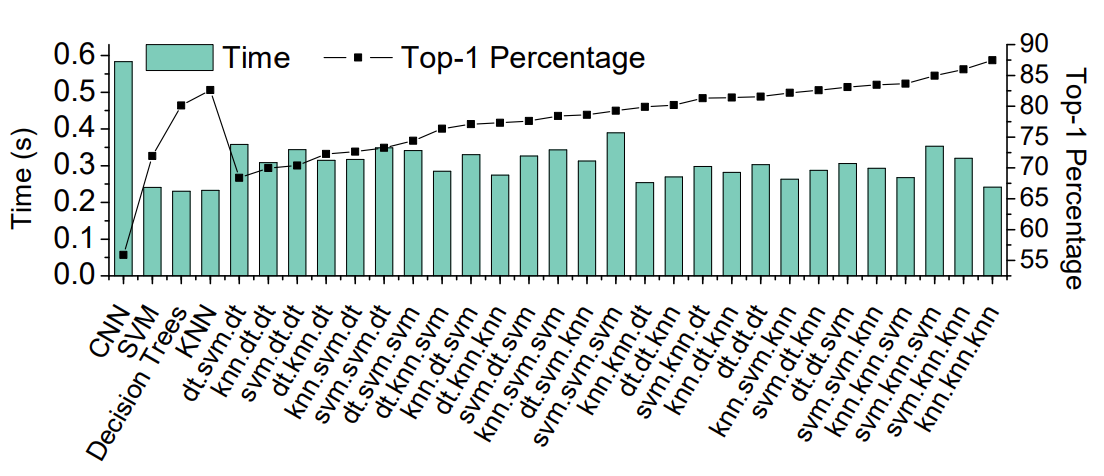
\includegraphics[width=0.7\textwidth]{report/figures/original_premodels.png}
	\caption{Premodel results in the original article. Premodel combinations show a large difference in accuracies and only small variation in time.}
	\label{fig:11a_orig}
\end{figure}
\begin{figure}
	\begin{subfigure}{.5\textwidth}
		\centering
		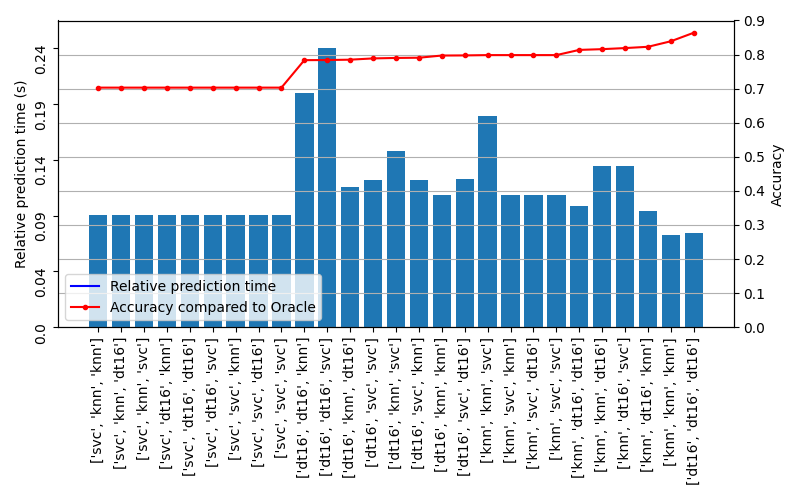
\includegraphics[width=0.99\textwidth]{report/figures/premodel_orderedByAcc_1000.png}
		\caption{Premodels trained on 1000 images}
	\end{subfigure}
	\begin{subfigure}{.5\textwidth}
		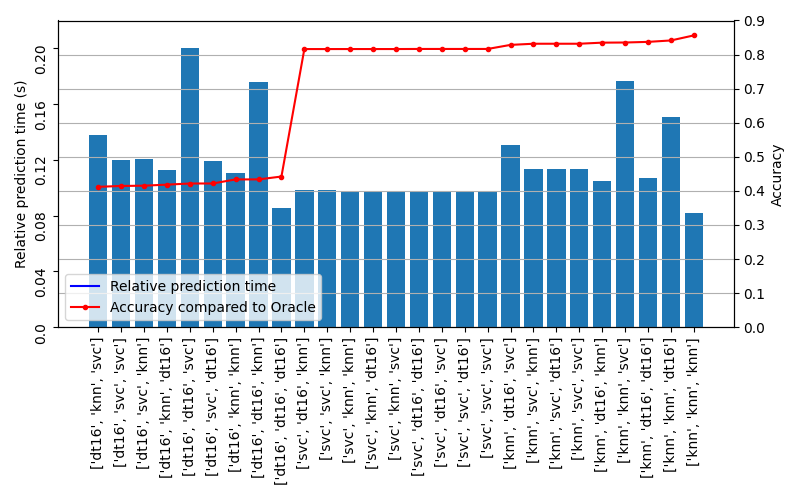
\includegraphics[width=0.99\textwidth]{report/figures/premodel_orderedByAcc_5000.png}
		\caption{Premodels trained on 5000 images}
	\end{subfigure}
	\caption{Our premodel results. Both accuracy and time show a large variation between different premodel combinations. Notably, large differences can arise from small changes such as number of training instances of the premodels. Less trained premodels are worse in well-distributing instances and result in lower inference speed.}
	\label{fig:11a_ours}
	
	
\end{figure}

\subsection{Machine translation}

\subsubsection{NMT models} % Idk, we should probably explain this situation first, since pretrained NMT models aren't availabe and the whole thing is quite sketchy

In the original article, the authors describe using 15 Tensorflow-NMT~\cite{luong17} models trained on WMT English-German dataset. Unlike the models used in the image classification part, pretrained models used for the machine translation part are not available online. In the original article, the authors mention number of layers and use of gnmt attention as the main difference between the models, but don't provide any other hyperparameters, therefore we assume they match the standard hyperparameters provided by Tensorflow-NMT.

Based on the original article, the models were trained on \textquote*[{\cite[p. 13]{marco2019optimizing}}]{WMT09-WMT14 English-German newstest dataset}. However, when we attempted to train Tensorflow-NMT models on that dataset, we were unable to reproduce the results, or even achieve any meaningful training, as shown in \figurename~\ref{fig:tf-nmt_paper_training}.

\begin{figure}[h]
	\centering
	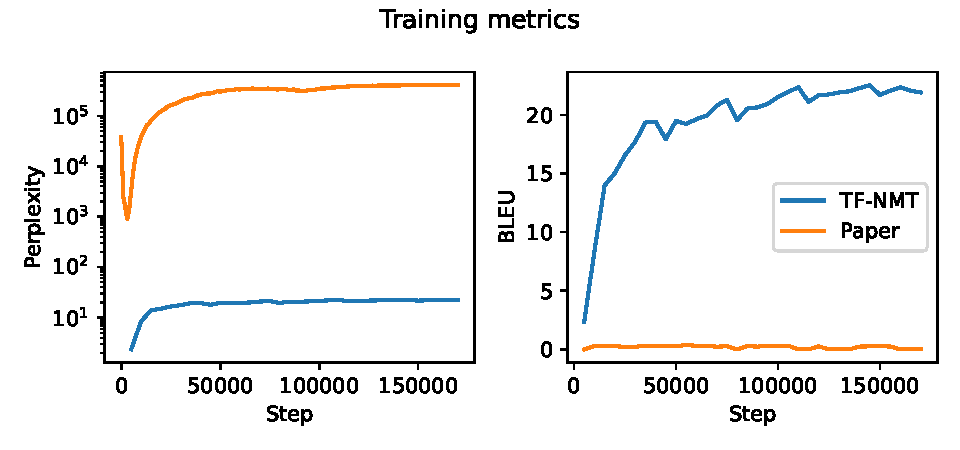
\includegraphics[width=0.75\textwidth]{figures/tf-nmt_paper_training.pdf}
	\caption{Comparison of training metrics when training the same Tensorflow-NMT model on WMT English-German newstest dataset (paper) and the whole WMT English-German dataset used by the Tensorflow-NMT authors (TF-NMT). It is clear that, at least without significant changes to the hyperparameters, the newstest dataset isn't sufficient to train Tensorflow-NMT models.}
	\label{fig:tf-nmt_paper_training}
\end{figure}

Because training the underlying NMT models isn't the primary focus of the original article, we decided to train the models following the standard WMT English-German training described in Tensorflow-NMT and train the four models used in the paper: 3\_layer, gnmt\_2\_layer, gnmt\_4\_layer, and gnmt\_8\_layer. We included hyperparameters and scripts we used to prepare both datasets and train our models with the code. We were unable to determine what the remaining 11 models used by the original authors were, as the original article simply states that they used 15 \textquote*[{\cite[p. 13]{marco2019optimizing}}]{models of varying sizes and architectures} based on Tensorflow-NMT in the model selection step.

\figurename~\ref{fig:nlp_scores} presents inference times along with the BLEU, ROUGE, and F1 scores for the evaluated models. While the overall accuracy is somewhat lower compared to the original article (\cite{marco2019optimizing}, Figure 10c), our 3\_layer model notably outperforms theirs, achieving a significantly higher scores than reported in the original study.

\begin{figure}[ht]
	\centering
	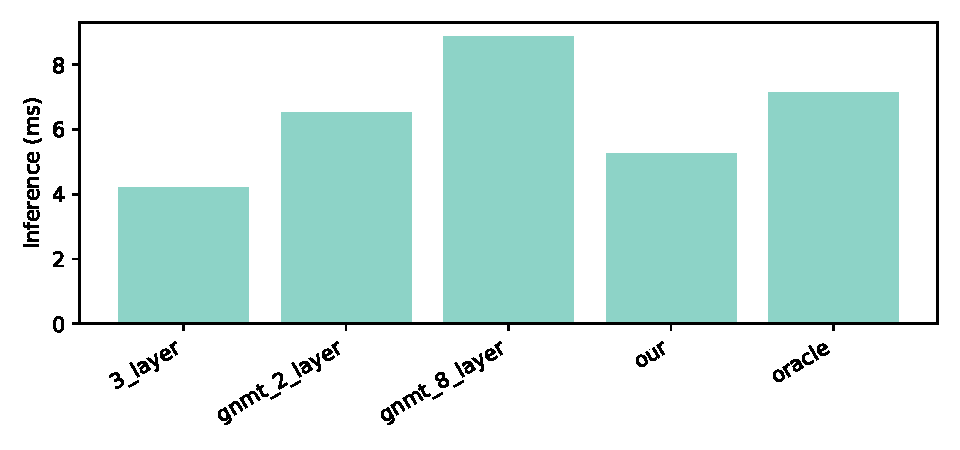
\includegraphics[width=0.45\textwidth]{figures/ml_inf_time.pdf}\quad
	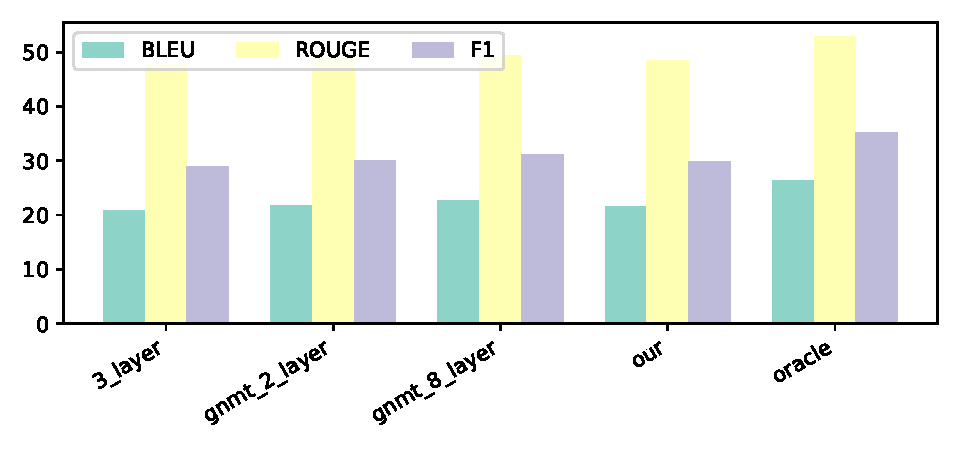
\includegraphics[width=0.45\textwidth]{figures/ml_inf_score.pdf}
	\caption{Inference times and scores of different models.}
	\label{fig:nlp_scores}
\end{figure}

\subsubsection{Premodel}
For the premodel for the machine translation part, the authors propose simple classifiers (KNN, DT, NB, SVM), either as a single multi-class classifier or a series of multiple binary classifiers of the same type. We also tested other classifiers available in the Scikit-learn library as it was unclear what the exact classifier implementations used by the original authors were, using 10-fold cross-validation. However, as with the NMT models, the dataset mentioned in the original paper simply wasn't enough to get any improvement over the baseline (\figurename~\ref{fig:nlp_premodels}). While we were able to train NMT models on the entire WMT dataset, we were unable to do so for the premodel as the time complexity for some of the models used in the paper is \(O(n^2)\) or even \(O(n^3)\).

It is unclear from the paper how the authors achieved their results, what part of the dataset they used, or what hyperparameters they used for each premodel in order to achieve their results. Therefore, we cannot directly compare our results to theirs, even though we did notice some improvement in inference time and F1 score comparable with Figure 11 in the original paper.

\begin{figure}[ht]
	\centering
	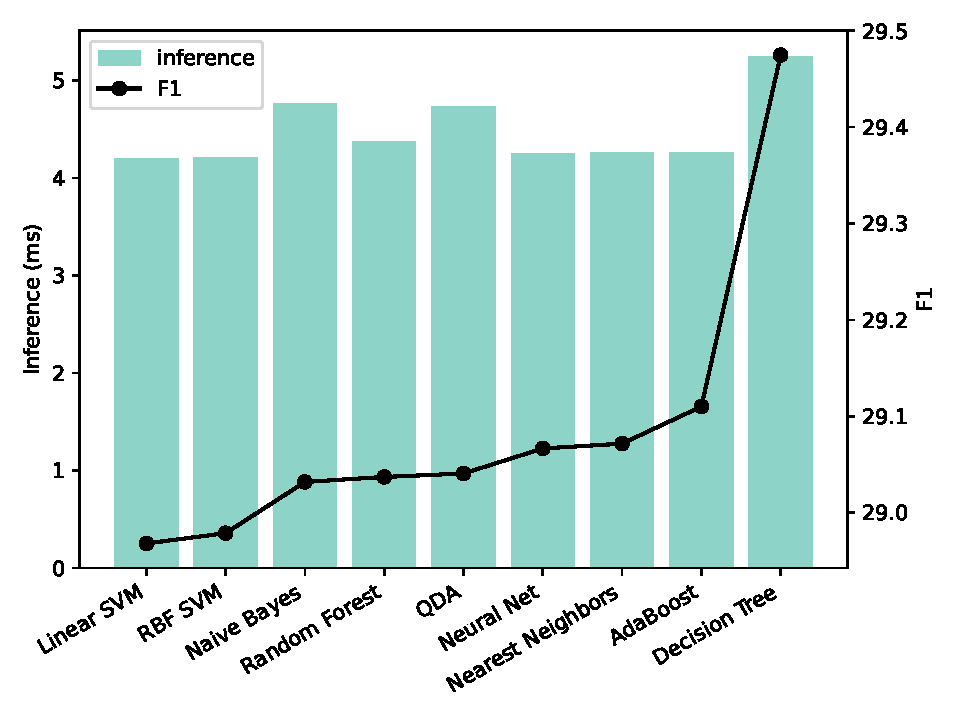
\includegraphics[width=0.75\textwidth]{figures/ml_inf_premodel.pdf}
	\caption{Comparison of different premodels. While there is improvement in inference time, the improvement in F1 score is only marginal, and much further from that reported by the original authors.}
	\label{fig:nlp_premodels}
\end{figure}

% We replicated the model selection algorithm, but without knowing what models the original authors considered in the model selection step, we weren't able to replicate the results for that part.

% ... at this point we got the translations generated by our models along with inference time for each sentence, and we can move to feature engineering and premodel, and try to replicate the main focus points of the original article


\subsection{Feature engineering}
\subsubsection{Image classification}

Our feature engineering efforts for image classification were guided by the features listed in the original study. However, due to the lack of specific details in the original paper, particularly regarding the algorithms used for keypoint detection, edge detection, and hue histogram calculation, we developed our own methods.

\paragraph{Keypoint Detection}
We employed the ORB (Oriented FAST and Rotated BRIEF) algorithm\supercite{Rublee2011ORBAE} for keypoint detection. This choice was based on ORB's efficiency and its ability to detect a large number of keypoints\footnote{\url{https://mikhail-kennerley.medium.com/a-comparison-of-sift-surf-and-orb-on-opencv-59119b9ec3d0}}.

\paragraph{Edge Detection and Analysis}
For edge detection, we used the Canny edge detector\supercite{canny1986computational} combined with contour analysis to calculate edge lengths. This resulted in our edge length histogram bins showing different correlation patterns compared to those reported in the original study. Similarly, for edge angles, we utilised the Sobel operator\supercite{kanopoulos1988design}, which also showed variations in correlation from the original findings.

\paragraph{Hue Histogram}
The calculation of the hue histogram was done using the HSV colour space conversion. We noted that our hue histogram bins were less correlated compared to those in the original study.

\paragraph{Aspect Ratio and Area by Perimeter}
For calculating the aspect ratio and area/perimeter ratio of the main object, we used contour detection methods. The specific algorithmic choices were made in the absence of detailed guidance from the original paper.

\paragraph{Correlation Analysis}
Our correlation analysis revealed significant differences from the original study. For instance, the correlation between different hue bins and between various edge angle bins diverged from the patterns reported in the original paper. These differences could potentially impact the effectiveness of the feature set in predictive modelling.

\paragraph{Visualisation of Correlations}
To effectively communicate our findings, we have included a heatmap of the Pearson correlation matrix of the features we computed (See Figure \ref{fig:correlation_matrix}). This visualisation provides an intuitive understanding of the relationships between different features in our implementation.

%Visualisation of Correlations: we computed 6 -> verjetno manjka (see Figure 6)?



%Figure 6: Ta bi lahko bil preko celotne širine, ker se slabo vidi. 
%TODO: poglej a je to kje popolnoma sesulo formatting (i love latex figures)

%Figure 6, 7: Jaz bi odstranil naslov Correlation Matrix.
\begin{figure}[h]
    \centering
	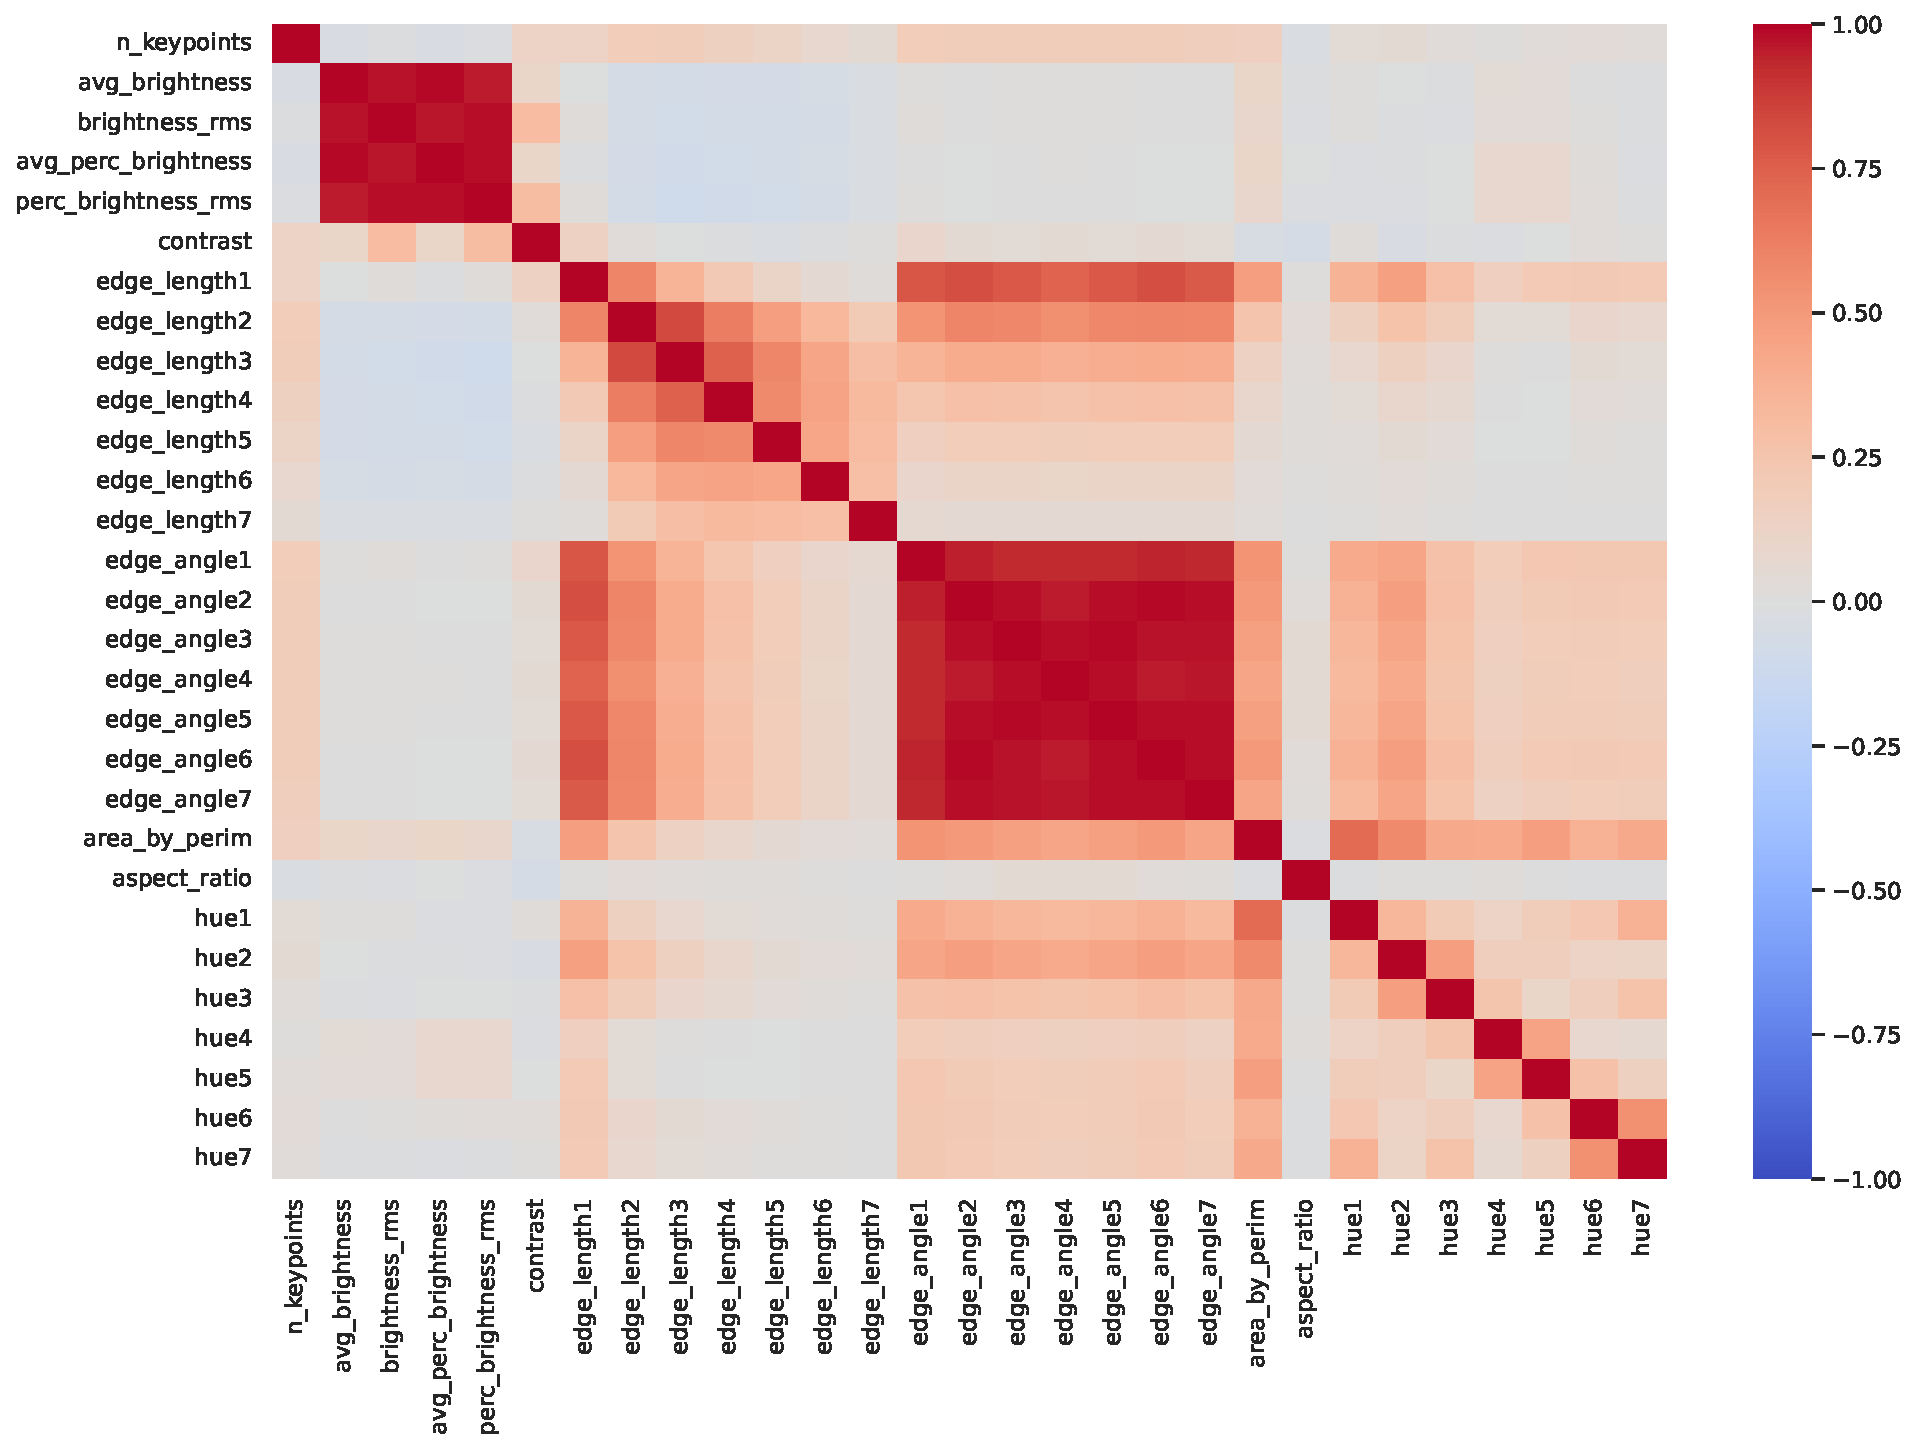
\includegraphics[width=0.9\textwidth]{report/figures/cv_corr_matrix1.pdf}
	\caption{Heatmap of the Pearson correlation matrix for the features in our image classification feature engineering.}
	\label{fig:correlation_matrix}
\end{figure}

%It's -> It is (se pojavi na več mestih)
It is important to note that these differences in correlations might influence the model's performance and generalizability, and our observations suggest areas where further research and clarification from the original authors might be beneficial.

\begin{table}[h]
	\centering
	\caption{Correlation values (absolute) of removed features to the kept ones for image classification.}
	\begin{tabular}{lll}
		\hline
		\textbf{Kept Feature} & \textbf{Removed Feature} & \textbf{Correl.} \\ \hline
		avg\_brightness       & brightness\_rms          & 0.98             \\
		                      & avg\_perc\_brightness    & 0.98             \\
		                      & perc\_brightness\_rms    & 0.96             \\
		edge\_angle1          & edge\_angle[2-7]         & 0.92 - 0.95      \\ \hline
	\end{tabular}
\end{table}



\subsubsection{Machine translation}
For the machine translation part we got much more similar results than the feature extraction part, despite a few problems.

\paragraph{Feature Selection and Challenges}
In our replication of the machine translation case study, we faced challenges primarily related to data and feature specification discrepancies in the original study. The original paper's dataset reference indicated 5k sentences, while the actual dataset contained 4.5 million samples. This discrepancy significantly influenced our approach to feature extraction and premodel training.

\paragraph{Feature Extraction Methodology}
For feature extraction, we focused on the 11 features listed in the original study (as per Table 7 in the original article), including \textit{n\_words}, \textit{n\_bpe\_chars}, \textit{avg\_bpe}, and others. However, due to the lack of specifics regarding the tokenizer and correlation metrics, we followed a similar methodology to that used for image classification, employing Pearson correlation and using Spacy and NLTK for our work.

\paragraph{Specific Features and Correlations}
Our analysis revealed several notable correlations: \textit{n\_words} correlated strongly with both \textit{n\_bpe\_chars} and \textit{n\_tokens}, while \textit{avg\_adj} correlated with \textit{avg\_sat\_adj}, with these adjective correlations remaining below the 0.9 threshold, thereby aligning with the correlation results reported in the original study. Another high correlation, which was excluded due to thresholding, was observed between \textit{avg\_bpe} and \textit{avg\_punc}, though the rationale behind this specific correlation remains unclear.

\paragraph{Bag of Words (BoW) Implementation}
Consistent with the original paper, we incorporated a BoW representation for each sentence. For that, we used Scikit-learn implementation with Chi-square feature reduction.

\paragraph{Correlation Matrix Visualisation}
To illustrate the feature correlations in our implementation, we included a heatmap of the Pearson correlation matrix, as shown in Figure \ref{fig:nlp_correlation_matrix}.
%Figure 6, 7: Jaz bi odstranil naslov Correlation Matrix.
\begin{figure}[h]
	\centering
	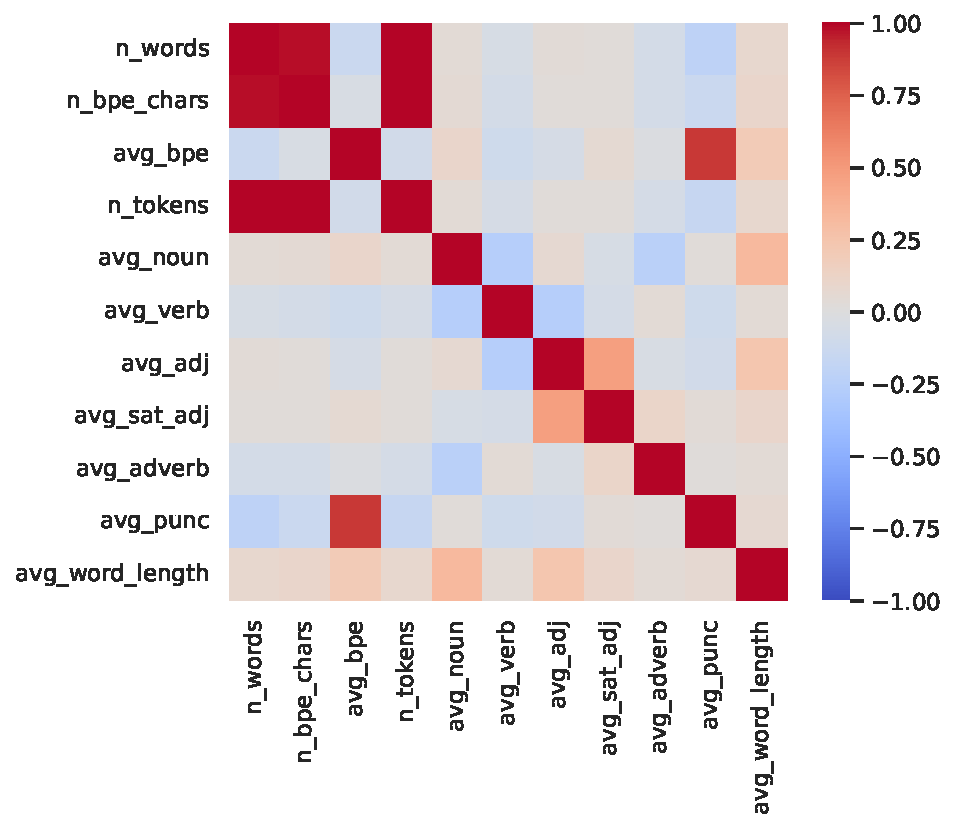
\includegraphics[width=0.7\textwidth]{figures/text_corr_matrix1.pdf}
	\caption{Heatmap of the Pearson correlation matrix for the features in our machine translation feature engineering.}
	\label{fig:nlp_correlation_matrix}
\end{figure}

This heatmap provides a visual representation of the relationships between different features in our MT feature engineering process, allowing for a direct comparison with the original study's findings.


% at Timotej and Marko: this is the other option:
%\section{Methodology}
%
%    \subsection{Computer vision}
%        \subsubsection{Base model}
%        \subsubsection{Feature engineering}
%        \subsubsection{Premodel}
%    
%    \subsection{Natural language processing}
%        \subsubsection{Base model}
%        \subsubsection{Feature engineering}
%        \subsubsection{Premodel}



\section{Results}
Our results strongly disagree with the original article. Our best-effort reconstruction of feature engineering and premodel pipeline shows some resemblance with the original results, but doesn't come close to the numbers shown in the original paper.

We observed noticeably larger differences in runtime, combined with strange behaviour in prediction accuracies, dependent on number of training samples for the premodels. These differences could stem from the fact that we have had to construct our own feature extraction process, as it is described in too vague a manner in the original article. Our results clearly reflect the attributes of the premodels, with lower runtime and lower accuracy sensibly following simpler predictors.

When reporting accuracies for premodels, we report accuracy compared to oracle model selector.

Regarding original authors' claims:
\begin{itemize}
	\item \textbf{Claim 1: image classification top-1 accuracy improvement.}
	      %with same best premodel -> with the same best premodel
	      Using this premodel pipeline, we succesfully surpassed best models with the same best premodel sequence.
	      
	\item \textbf{Claim 2: image classification reduction in inference time.}
	      
	      Using any premodel combination significantly speeds up image classification, as opposed to always using the "strongest" model. Notably, we observed even larger speed-up that expected, from almost 3x with the worst premodel combination up to almost 7x.
	      
	\item \textbf{Claim 3: machine translation reduce inference time without affecting accuracy.}
	      
	      While different premodels did reduce inference time close to what has been reported in the original paper, they didn't show any improvement in accuracy over the baseline 3\_layer model due to a large number of misclassified sentences. However, it is worth noting that our 3\_layer model achieves marginally worse overall performance than gnmt\_8\_layer model, and since the models are much more similar in architecture than those used for image classification we weren't expecting to see any major improvement.
	      
\end{itemize}



\section{Discussion}
%Trying to replicate the methods and results described in the paper was very much about connecting the dots and filling the blanks. -> To bi lahko povedali na malo bolj formalen način. V smislu, da ni bilo dovolj informacij za reprodukcijo, zato ste določene korake dopolnili po lastni presoji.

Due to insufficient information for reproduction of methods and results described in the paper, we have estimated the procedures used as best as we could. While the original paper clearly notes what models and images were used for image classification task, with both readily available online, it fails to do the same for machine translation part, 
%or does it with plenty of ambiguity. -> or is ambigious.
or is it ambiguous. It is also unclear how the datasets for training and evaluation of the premodels were obtained, as neither the data used nor the exact code to generate the data are available. The authors provided an extensive report on feature selection and evaluation, and made great effort justifying their results. 
%However, we could not verify any of that -> However, we could not replicate those results 
However, we could not replicate those results, as even our best-effort results only vaguely aligned with the original paper and never matched the improvement claimed by the authors.

%We believe that a well written research article should be entirely reproducible. Unfortunately, without detailed information, it is challenging to replicate the results, and we had to explore numerous alternative approaches to approximate the outcomes presented in the original article. This lack of transparency raises concerns about the reliability of the reported findings and scientific correctness of methods used by the authors. -> prvi del tega odstavka je samoumeven, drugi del pa je tudi že bil v bistvu povedan (med vrsticami in direktno). Jaz bi izpustil ta odstavek.

%We believe that a well-written research article should be entirely reproducible. Unfortunately, without detailed information, it is challenging to replicate the results, and we had to explore numerous alternative approaches to approximate the outcomes presented in the original article. This lack of transparency raises concerns about the reliability of the reported findings and scientific correctness of methods used by the authors.